\chapter{Data Science in datengesteuerten Organisationen}

Inhalt dieses Kapitels ist die Darstellung des aktuellen Stands der Forschung zur Eingliederung von Data Science Teams in datengesteuerten Organisationen.
Damit wird verfolgt, ein aktuelles Zielbild annäherungsweise zu konkretisieren, um in weiteren Kapiteln auf die Möglichkeiten zur Integration einzugehen.

Eine Herausforderung entsteht bereits dabei, dass datengesteuerte Organisationen, in der Fachsprache als \textit{data driven Organizations} bezeichnet, einer Vielfalt an Definitionen unterliegen. \footcite[prenote][postnote]{(several definitons of DDOs)}
\Citeauthor*{Fabijan.2017} definierte z. B., dass datengesteuerte Organisationen Daten akquirieren, verarbeiten und Datenvorteile in einer zeitlich angebrachten Art und Weise nutzen, um Effizienzgewinne zu erzeugen, neuartige Produkte zu entwickeln und sich durch die Wettbewerbslandschaft zu navigieren. \footcite[prenote][postnote]{DDO definition}
% insert second definition
Ein gemeinsames Verständnis der Definitionen besteht in dem Prozess des Sammeln von Daten, der Gewinnung von Erkenntnissen durch Analysen und dem Treffen von Entscheidungen basierend auf den erzielten Analyseergebnissen. \footcite[prenote][postnote]{looking into DDO definitions}

Einer der wichtigsten Aspekte einer datengesteuerten Organisation ist die Manifestation einer datengesteuerten Kultur. \footcite[prenote][postnote]{data-driven culture}
Dessen Antrieb ist es, Daten nicht nur den Analytic-Abteilungen oder dem leitenden Management vorbehalten sind, sondern so weit wie rechtlich möglich, jedem Organisationsmitglied zur Verfügung gestellt werden sollte. \footcite[prenote][postnote]{ddos democratize data}
Dieser Umgang würde es ermöglichen, alle Arten der Analyse (deskriptiv, prädiktiv, präskriptiv) auf allen Ebenen der Organisation (operativ, taktisch, strategisch) einzusetzen. \footcite[prenote][postnote]{typees of analytics}
In der bisherigen Praxis wird von diesen Möglichkeiten jedoch nur ein Teil angewendet. \footcite[prenote][postnote]{typees}
Weitere Aspekte einer datengesteuerten Organisation konnten durch die Forschung von \Citeauthor*{Marius Hupperz, Inan Gür et al. 2021} identifiziert werden.
Für den untersuchten Aspekt der Data Science ist erkannt worden, dass der Wertbeitrag durch Transparenz, zielgerichtetem Marketing oder automatisierten informierten Entscheidungen zu Wettbewerbsvorteilen führen kann, jedoch keinen unmittelbaren Einflüsse auf die Vermögenswerte ausüben. \footcite[prenote][postnote]{data science brings value}
Zusätzlich kann Einrichtung einer Digitalisierungsabteilung zwar die Transformation zum datengesteuerten Unternehmen unterstützen, jedoch durch das alleinige Einrichten von Data Science Abteilungen keine Geschäftserkenntnisse aus Daten zu erzeugen. \footcite[prenote][postnote]{data science teams}
Alle weiteren Aspekte aus der strukturierten Literaturanalyse von datengesteuerten Organisationen sind in folgender Mindmap dargestellt:

\begin{figure}[htb]
    \centering
    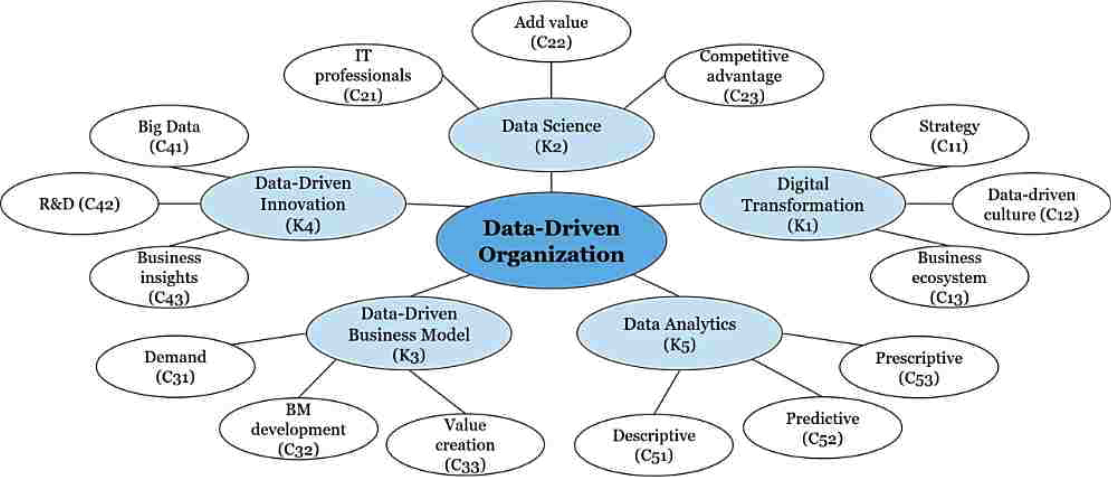
\includegraphics[width=0.95\textwidth]{graphics/ddo aspects.png}
    \caption{In der Literatur beschriebene Aspekte von datengesteuerten Organisationen}
    \label{fig:DDOs aspects}
\end{figure}

Zur praktischen Umsetzung von datengesteuerten Unternehmen führten \Citeauthor*{Zhang, Muller et al. 2020} eine Online Befragung mit insgesamt 183 Teilnehmenden aus der Data Science durch.
Da alle Beteiligten der Umfrage aus der IBM als ein IT-Konzern stammen, ist die Umfrage zwar nicht repräsentativ für alle Organisationen, zeigt jedoch ein signifikantes Bild über den Aufbau und die Zusammenarbeit von Data Science Abteilungen.
